%%%%%%%%%%%%%%%%%%%%%%%%%%%%%%%%%%%%%%%%%
% Wenneker Article
% LaTeX Template
% Version 2.0 (28/2/17)
%
% This template was downloaded from:
% http://www.LaTeXTemplates.com
%
% Authors:
% Vel (vel@LaTeXTemplates.com)
% Frits Wenneker
%
% License:
% CC BY-NC-SA 3.0 (http://creativecommons.org/licenses/by-nc-sa/3.0/)
%
% Adapted for COMS30007 by Carl Henrik Ek
%
%%%%%%%%%%%%%%%%%%%%%%%%%%%%%%%%%%%%%%%%%

%----------------------------------------------------------------------------------------
%	PACKAGES AND OTHER DOCUMENT CONFIGURATIONS
%----------------------------------------------------------------------------------------

\documentclass[10pt, a4paper, twocolumn]{article} % 10pt font size (11 and 12 also possible), A4 paper (letterpaper for US letter) and two column layout (remove for one column)

%%%%%%%%%%%%%%%%%%%%%%%%%%%%%%%%%%%%%%%%%
% Wenneker Article
% Structure Specification File
% Version 1.0 (28/2/17)
%
% This file originates from:
% http://www.LaTeXTemplates.com
%
% Authors:
% Frits Wenneker
% Vel (vel@LaTeXTemplates.com)
%
% License:
% CC BY-NC-SA 3.0 (http://creativecommons.org/licenses/by-nc-sa/3.0/)
%
% Adapted for COMS30007 by Carl Henrik Ek
%
%%%%%%%%%%%%%%%%%%%%%%%%%%%%%%%%%%%%%%%%%

%----------------------------------------------------------------------------------------
%	PACKAGES AND OTHER DOCUMENT CONFIGURATIONS
%----------------------------------------------------------------------------------------

\usepackage[english]{babel} % English language hyphenation

\usepackage{microtype} % Better typography

\usepackage{amsthm} % Math packages for equations
\usepackage{amsmath}
\usepackage{amssymb}
\usepackage{mathtools}
\usepackage{bm}
\usepackage{xfrac}
\usepackage{resizegather}



\usepackage[svgnames]{xcolor} % Enabling colors by their 'svgnames'

\usepackage[hang, small, labelfont=bf, up, textfont=it]{caption} % Custom captions under/above tables and figures

\usepackage{booktabs} % Horizontal rules in tables

\usepackage{lastpage} % Used to determine the number of pages in the document (for "Page X of Total")

\usepackage{graphicx} % Required for adding images

\usepackage{enumitem} % Required for customising lists
\setlist{noitemsep} % Remove spacing between bullet/numbered list elements

\usepackage{sectsty} % Enables custom section titles
\allsectionsfont{\usefont{OT1}{phv}{b}{n}} % Change the font of all section commands (Helvetica)

%----------------------------------------------------------------------------------------
%	MARGINS AND SPACING
%----------------------------------------------------------------------------------------

\usepackage{geometry} % Required for adjusting page dimensions

\geometry{
	top=1cm, % Top margin
	bottom=1.5cm, % Bottom margin
	left=2cm, % Left margin
	right=2cm, % Right margin
	includehead, % Include space for a header
	includefoot, % Include space for a footer
	%showframe, % Uncomment to show how the type block is set on the page
}

\setlength{\columnsep}{7mm} % Column separation width

%----------------------------------------------------------------------------------------
%	FONTS
%----------------------------------------------------------------------------------------

\usepackage[T1]{fontenc} % Output font encoding for international characters
\usepackage[utf8]{inputenc} % Required for inputting international characters

\usepackage{XCharter} % Use the XCharter font

%----------------------------------------------------------------------------------------
%	HEADERS AND FOOTERS
%----------------------------------------------------------------------------------------

\usepackage{fancyhdr} % Needed to define custom headers/footers
\pagestyle{fancy} % Enables the custom headers/footers

\renewcommand{\headrulewidth}{0.0pt} % No header rule
\renewcommand{\footrulewidth}{0.4pt} % Thin footer rule

\renewcommand{\sectionmark}[1]{\markboth{#1}{}} % Removes the section number from the header when \leftmark is used

%\nouppercase\leftmark % Add this to one of the lines below if you want a section title in the header/footer

% Headers
\lhead{} % Left header
\chead{\textit{\thetitle}} % Center header - currently printing the article title
\rhead{} % Right header

% Footers
\lfoot{} % Left footer
\cfoot{} % Center footer
\rfoot{\footnotesize Page \thepage\ of \pageref{LastPage}} % Right footer, "Page 1 of 2"

\fancypagestyle{firstpage}{ % Page style for the first page with the title
	\fancyhf{}
	\renewcommand{\footrulewidth}{0pt} % Suppress footer rule
}

%----------------------------------------------------------------------------------------
%	TITLE SECTION
%----------------------------------------------------------------------------------------

\newcommand{\authorstyle}[1]{{\large\usefont{OT1}{phv}{b}{n}\color{DarkRed}#1}} % Authors style (Helvetica)

\newcommand{\institution}[1]{{\footnotesize\usefont{OT1}{phv}{m}{sl}\color{Black}#1}} % Institutions style (Helvetica)

\usepackage{titling} % Allows custom title configuration

\newcommand{\HorRule}{\color{DarkGoldenrod}\rule{\linewidth}{1pt}} % Defines the gold horizontal rule around the title

\pretitle{
	\vspace{-30pt} % Move the entire title section up
	\HorRule\vspace{10pt} % Horizontal rule before the title
	\fontsize{32}{36}\usefont{OT1}{phv}{b}{n}\selectfont % Helvetica
	\color{DarkRed} % Text colour for the title and author(s)
}

\posttitle{\par\vskip 15pt} % Whitespace under the title

\preauthor{} % Anything that will appear before \author is printed

\postauthor{ % Anything that will appear after \author is printed
	\vspace{10pt} % Space before the rule
	\par\HorRule % Horizontal rule after the title
	\vspace{20pt} % Space after the title section
}

%----------------------------------------------------------------------------------------
%	ABSTRACT
%----------------------------------------------------------------------------------------

\usepackage{lettrine} % Package to accentuate the first letter of the text (lettrine)
\usepackage{fix-cm}	% Fixes the height of the lettrine

\newcommand{\initial}[1]{ % Defines the command and style for the lettrine
	\lettrine[lines=3,findent=4pt,nindent=0pt]{% Lettrine takes up 3 lines, the text to the right of it is indented 4pt and further indenting of lines 2+ is stopped
		\color{DarkGoldenrod}% Lettrine colour
		{#1}% The letter
	}{}%
}

\usepackage{xstring} % Required for string manipulation

\newcommand{\lettrineabstract}[1]{
	\StrLeft{#1}{1}[\firstletter] % Capture the first letter of the abstract for the lettrine
	\initial{\firstletter}\textbf{\StrGobbleLeft{#1}{1}} % Print the abstract with the first letter as a lettrine and the rest in bold
}

%----------------------------------------------------------------------------------------
%	BIBLIOGRAPHY
%----------------------------------------------------------------------------------------

\usepackage[backend=bibtex,style=authoryear]{biblatex} % Use the bibtex backend with the authoryear citation style (which resembles APA)

\addbibresource{example.bib} % The filename of the bibliography

\usepackage[autostyle=true]{csquotes} % Required to generate language-dependent quotes in the bibliography
 % Specifies the document structure and loads requires packages

\usepackage{lipsum}

%----------------------------------------------------------------------------------------
%	ARTICLE INFORMATION
%----------------------------------------------------------------------------------------

\title{Models} % The article title

\author{
	\authorstyle{Justin Salmon\textsuperscript{1} and George Lancaster\textsuperscript{2}} % Authors
	\newline\newline % Space before institutions
	\textsuperscript{1}\institution{wr18313}\\ % Institution 1
	\textsuperscript{2}\institution{qv18258} % Institution 2
}


\date{\today} % Add a date here if you would like one to appear underneath the title block, use \today for the current date, leave empty for no date

%----------------------------------------------------------------------------------------

\begin{document}

\maketitle % Print the title

\thispagestyle{firstpage} % Apply the page style for the first page (no headers and footers)

%----------------------------------------------------------------------------------------
%	ABSTRACT
%----------------------------------------------------------------------------------------
\lettrineabstract{Lorem ipsum dolor sit amet, consectetur adipiscing elit. Fusce maximus nisi ligula. Morbi laoreet ex ligula, vitae lobortis purus mattis vel. Vestibulum ante ipsum primis in faucibus orci luctus et ultrices posuere cubilia Curae; Donec ac metus ut turpis mollis placerat et nec enim. Duis tristique nibh maximus faucibus facilisis. Praesent in consequat leo. Maecenas condimentum ex rhoncus, elementum diam vel, malesuada ante.}

%----------------------------------------------------------------------------------------
%	ARTICLE CONTENTS
%----------------------------------------------------------------------------------------

\section{The Prior}

\subsection{Theory}

\subsubsection*{Question 1.1}

A Gaussian likelihood encodes the inherent noise present in most real-world data. In other words, most probabilistic processes in nature tend to be noisy, and that noise tends to follow a Gaussian distribution. Hence this is generally a good place to start.

Noise in input data - assume noise is gaussian -> implies gaussian likelihood

\subsubsection*{Question 1.2}

Choosing a spherical covariance matrix essentially means that we are assuming that the input noise is going to be equal in all directions, i.e. the distribution is equally likely to deviate from the mean in all directions. Again, this is a good place to start. Choosing a non-spherical covariance would imply that we know something in advance about the relationship between the input and output, which is not true in this case.

\subsubsection*{Question 2}

TODO
The covariance matrix would not be in terms of the identity matrix (for some reason). We would have non-zero values in the offset diagonals which correspond to the correlations between different things.

\subsubsection{Linear Regression}

\subsubsection*{Question 3}

\begin{align}
  p(\mathbf{Y} | \mathbf{X}, \mathbf{W}, \beta) = \prod_{i=0}^N \mathcal{N} (y_i | \mathbf{W}^T\phi(x_i), \beta^-1)
\end{align}

\subsubsection*{Question 4}

A distribution is conjugate to another if they both take the same algebraic form, i.e. are in the same probability distribution family. For example, Gaussians are conjugate to each other, and the conjugate to a Bernoulli distribution is a Beta distribution. Conjugates are used as a convenience used to avoid calculating the denominator in Baye's rule (the evidence) which can often be a tricky integral. If the prior and likelihood are conjugate, then their product will be proportional to the posterior.

\subsubsection*{Question 5}

Euclidean distance from the mean

X appears only in the gaussian exponential part

\subsubsection*{Question 6}

Derive posterior mean and covariance, start at conjugacy. Watch video https://www.youtube.com/watch?v=nrd4AnDLR3U

\subsubsection{Non-parametric Regression}

\subsubsection*{Question 7}

Non-parametric: not defining parameters, just using what we know about the current data to classify new data points
The simplest example of a. non-parementric model is a K-nearest neieghbour nmodel.
The data are the parameters

Interpretability: 

\subsubsection*{Question 8}

This prior represents the space of all possible functions. 

We think that smooth functions are more likely, but non-smooth functions e.q. sawtooth are non-zero but very unlikely

\subsubsection*{Question 9}

All possible functions? Yes, but some are more likely than others

\subsubsection*{Question 10}

\begin{align}
  p(\mathbf{Y},\mathbf{X}, f, \mathbf{\theta}) = p(Y|f)p(F|X,\theta)p(X)p(\theta)
\end{align}

TODO draw graphical model

Assumptions:
- X and theta do not depend on anything
- F depends on theta and X
- Y depends on F

\subsubsection*{Question 11}

The marginal in Eq. 2 connects the prior and the data because we now have a way to directly generate Y values given X and theta value without knowing the actual form of f.

The uncertainty "filters" through this ...
We are uncertain about the function, so by marginalising it out the uncertainty gets "baked in" to Y.

The fact that $\mathbf{\theta}$ is left on the LHS of the expression after marginalisation means that it is needed (along with x) to calculate Y. Y is dependent on theta.

Use the model diagram to help?

Marginalisation is the average of some distributions
It is a weighted average of some functions, based on how likely each function is

\subsection{Practical}

\subsubsection{Linear Regression}

\subsubsection*{Question 12.1}

\begin{figure}[htbp]
\centerline{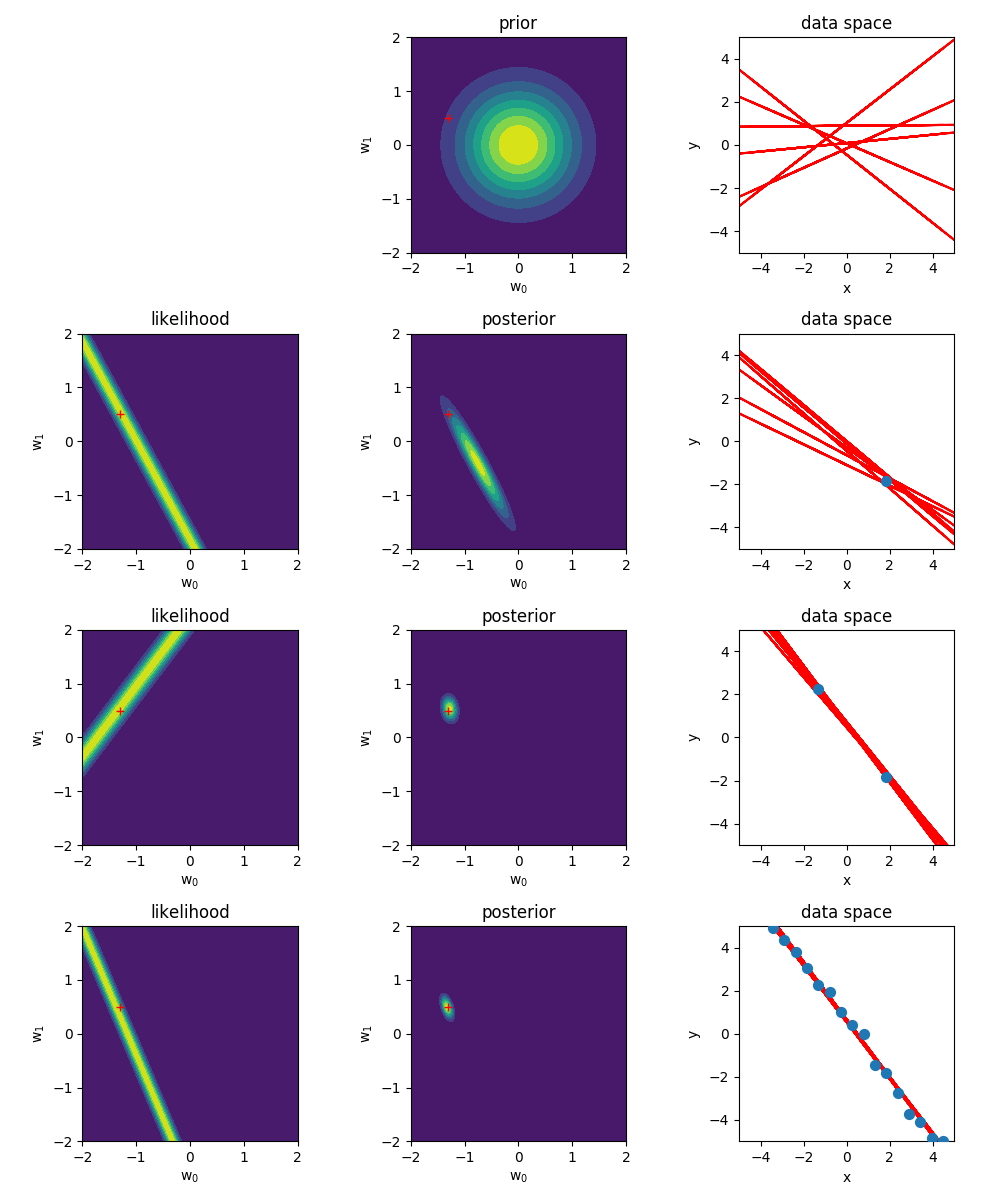
\includegraphics[width=8cm]{q12.png}}
\caption{TODO.}
\label{fig2}
\end{figure}

\section{Posterior}

\subsubsection*{Question 15}

Assumptions are what we assume to be true about something. They are a starting point, a way of being able to move forward from a point given no data about the problem. If we had all the data in the world, we would need no assumptions.

Use the assumptions to formulate a prior, use the prior to formulate your beliefs. Believe that the smooth lines are more likely. Prefer straight or flat lines.

Assumptions and preferences are very much similar. Preferences are the assumptions you want to use the most because it is easier exploiting conjugacy)

Beliefs inform assumptiosn (gaussian mean 0)

\begin{align}
  f &\sim \mathcal{N}\left(\boldsymbol{0},\beta^{-1}\mathbf{I}\right)\\
  \beta &\sim \Gamma(a)
\end{align}

\section{Evidence}

%----------------------------------------------------------------------------------------
%	BIBLIOGRAPHY
%----------------------------------------------------------------------------------------

\printbibliography[title={Bibliography}] % Print the bibliography, section title in curly brackets

%----------------------------------------------------------------------------------------

\end{document}
